\begin{figure}[h!]
  \begin{minipage}[c]{0.45\textwidth}
    \caption{
      \textbf{In theory, the smoothing approach should be more robust than the bin approach.} Both panels depict the same mutation location data for a hypothetical chromosome, with the black dots below the x-axis representing the true location of mutations. By binning the genome by convention, one counts the number of mutations in each yellow bin. The obtained GLE data is then the yellow dots on top of each bin. This binned GLE data changes when shifting the bin boundaries from panel (a) to panel (b). Mutations on the right hand side of the last bin (10$^{th}$ bin) are forcefully removed. By smoothing the genome, GLE data is the same for both panels. The smoothing method also allows inclusion of mutations outside the last bins.
    } \label{fig:mutdistribution_demo}
  \end{minipage}\hfill
  \begin{minipage}[c]{0.52\textwidth}
    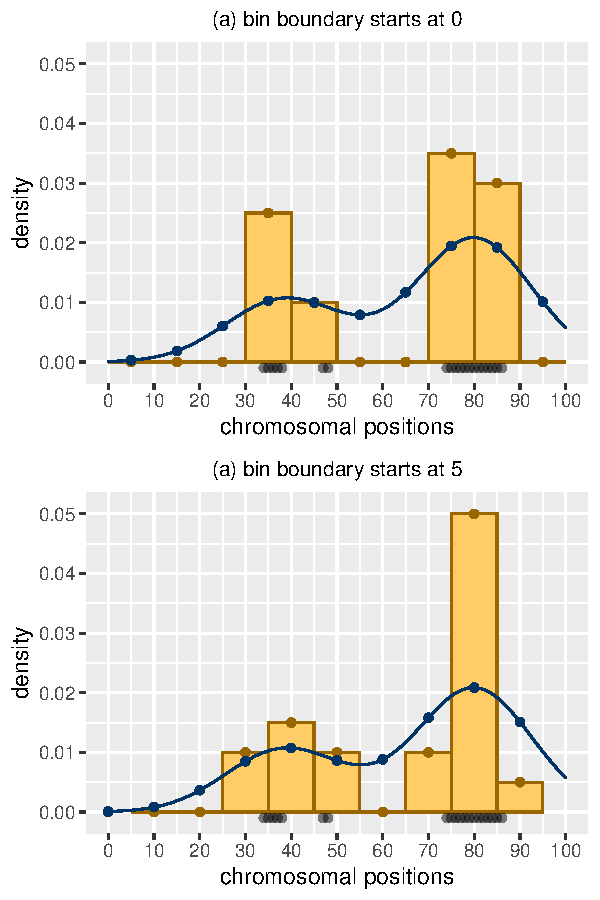
\includegraphics[width=\textwidth]{graphics/mutdistribution_demo.pdf}
  \end{minipage}
\end{figure}
